\documentclass{article}
\usepackage{geometry}
\usepackage[utf8]{inputenc}
\usepackage[T2A]{fontenc}
\usepackage{graphicx}
\usepackage{fancyhdr}
\usepackage{subfigure}
\usepackage{float}
\usepackage{fixltx2e}
\pagestyle{fancy}



% Set your name and assignment details here
\newcommand{\studentName}{Stefan du Toit, Benjamin Stephenson}
\newcommand{\courseTitle}{ECL1}
\newcommand{\assignmentTitle}{Exercise 05}
\newcommand{\bracketsub}[2]{%
  \left[ #1 \right]_{\text{#2}}%
}

% Header
\fancyhead[L]{\studentName}
\fancyhead[R]{\assignmentTitle}
\renewcommand{\headrulewidth}{0.4pt}

% Footer
\fancyfoot[L]{\today}
\fancyfoot[C]{}
\fancyfoot[R]{Page \thepage}
\renewcommand{\footrulewidth}{0.4pt}

\geometry{
  top=0.7in,
  bottom=0.7in,
  left=1in,
  right=1in
}
\begin{document}

\begin{titlepage}
    \begin{center}
        \vspace*{1cm}
        
        \Huge \textbf{\courseTitle}
        
        \LARGE \assignmentTitle
        
        \vspace{0.5cm}
     
        
        \vspace{1.5cm}
        
        \Large \textbf{\studentName}
        
        \vfill
        
  
        
        \vspace{0.8cm}
        
     
        
        \vspace{1cm}
        
        \Large UZH
        
    \end{center}
\end{titlepage}

\section{}		%1
\subsection{}
a) \\
b) \\
c) \\
This is not a CFG. It has a string (i.e. a terminal) on the left, which is not allowed. There has to be a single non-terminal on the left of the arrow fo rit to be a CFG.  \\
d) \\
This is a CFG. It has one non-terminal symbol on the left and one terminal followed by a non-terminal symbol on the right. Since the non-terminal symbol is the same on both sides of the arrow this represents recursiveness. \\ \\
e) \\
This is a CFG. The non-terminal A can derive itself or the non-terminal B or C. \\
f) \\
This is a CFG. The non-terminal B can derive the terminal a. As it only has the one terminal symbol on the right, it is also in Chomsky normal form.\\

\subsection{}
\section{} % 2
\section{} % 3
\section{} % 4
\subsection{}

a) \\

\subsubsection{}	%sentence 1
Sentence 1: The old man the boat. \\
\begin{figure}[H]
  \centering
  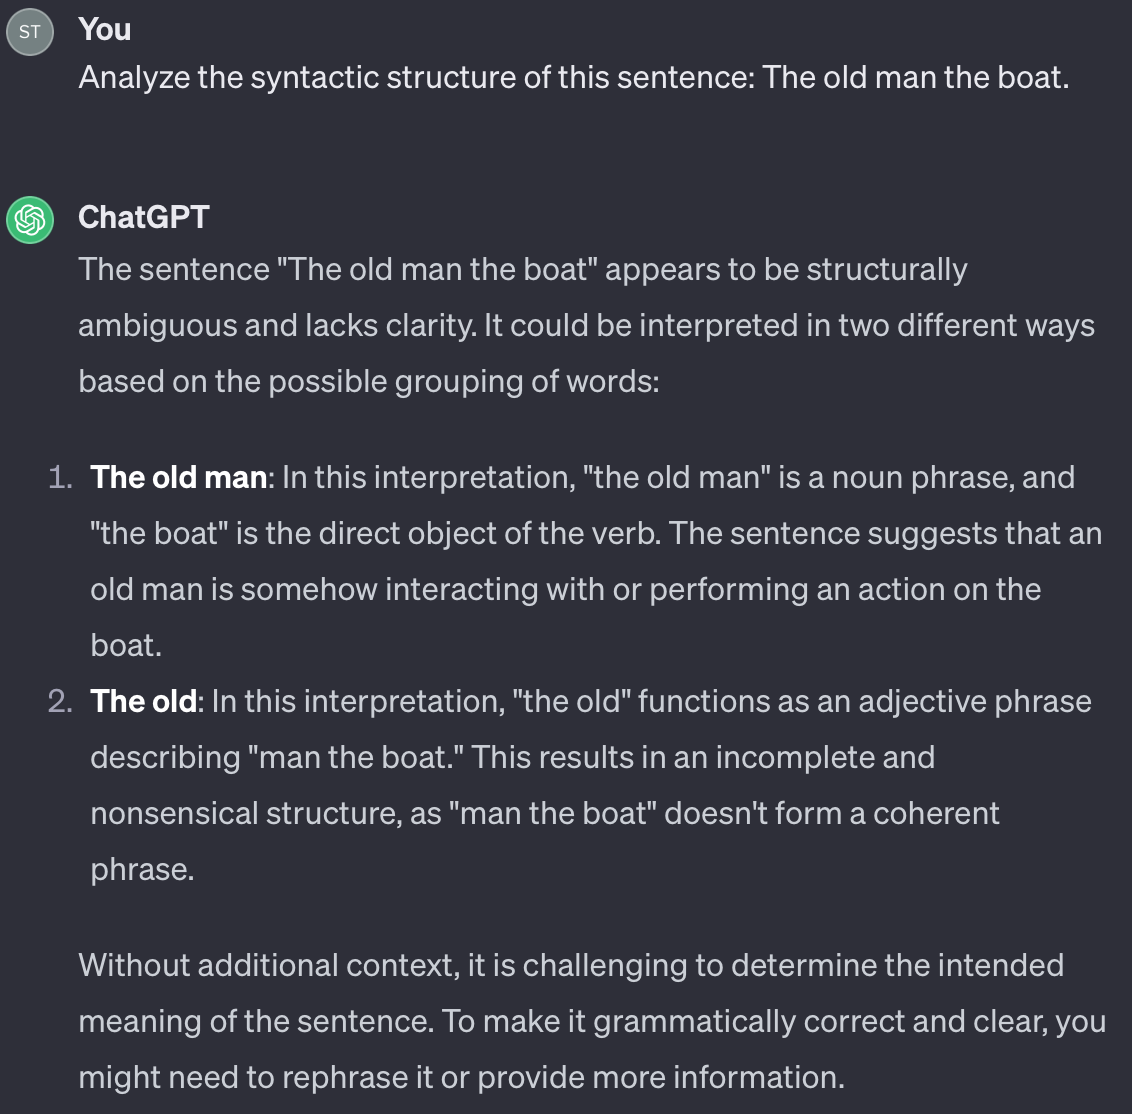
\includegraphics[width=0.6\textwidth]{4.1a1.png} 
  \caption{sentence 1}
\end{figure}


Sentence 1 is clearly wrong. The only way to interpret this sentence is: \\
\bracketsub{the\ old}{subject}\bracketsub{man}{verb}\bracketsub{the\ boat}{object} \\

It is understandable that GPT got this wrong because the verb 'to man' isn't commonly used, and using 'the old' as a nominal phrase is also unexpected. \\
\subsubsection{}	%sentence 2
Sentence 2: "The weary men manned the old boat on the tumultuous sea." \\
\begin{figure}[H]
  \centering
  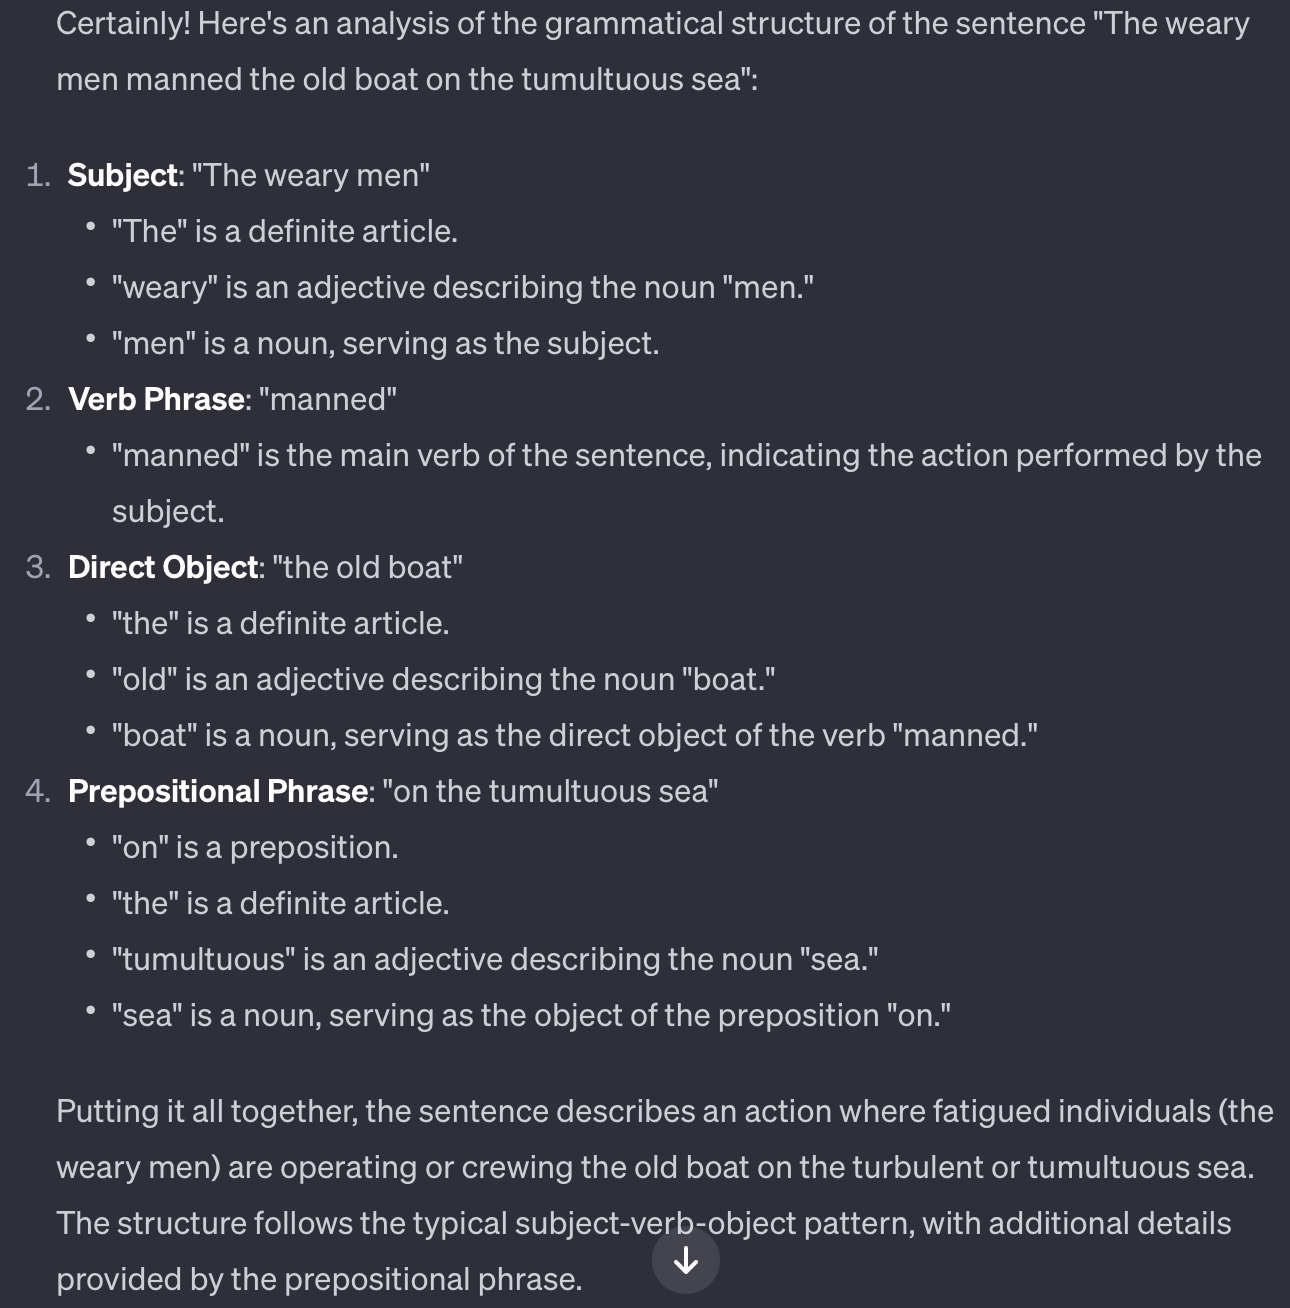
\includegraphics[width=0.6\textwidth]{4.1a2.png} 
  \caption{sentence 2}
\end{figure}


Sentence 2 was parsed perfectly. \\
\subsubsection{}	%sentence 3
Sentence 3: "The weary did man their boat on the tumultuous sea." \\
\begin{figure}[H]
  \centering
  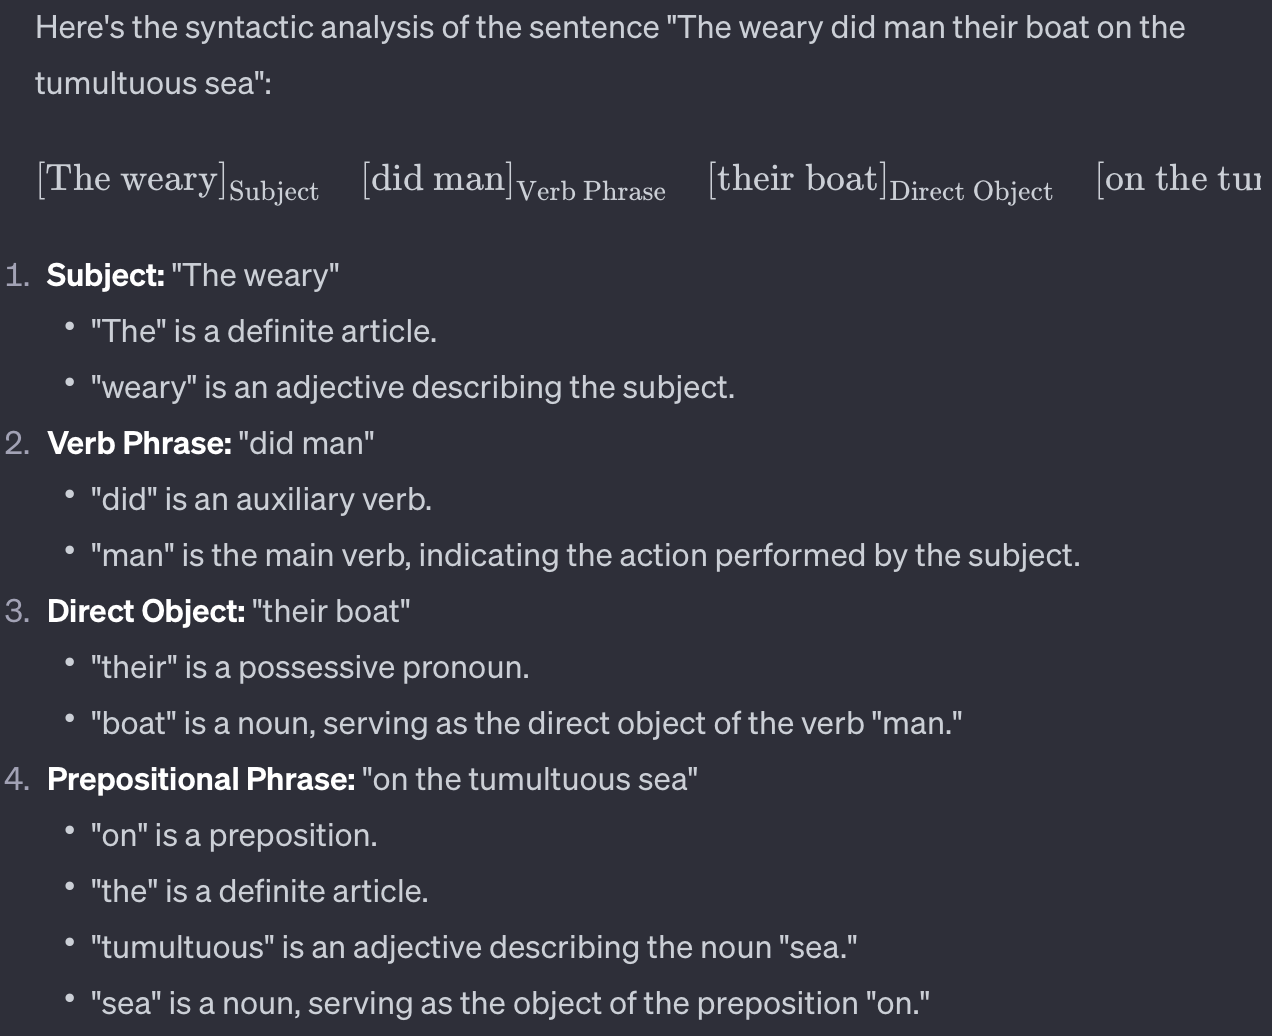
\includegraphics[width=0.6\textwidth]{4.1a5.png} 
  \caption{sentence 3}
\end{figure}


Sentence 3 was parsed perfectly. The only little mistake is that they say 'weary' is an adjective, although in this context it is actually a noun. But you could argue that it is an adjective to the implicit noun (people, men etc) \\
\subsubsection{}	%sentence 4
Sentence 4: "That we may fail is that which scares us most." \\
\begin{figure}[H]
  \centering
  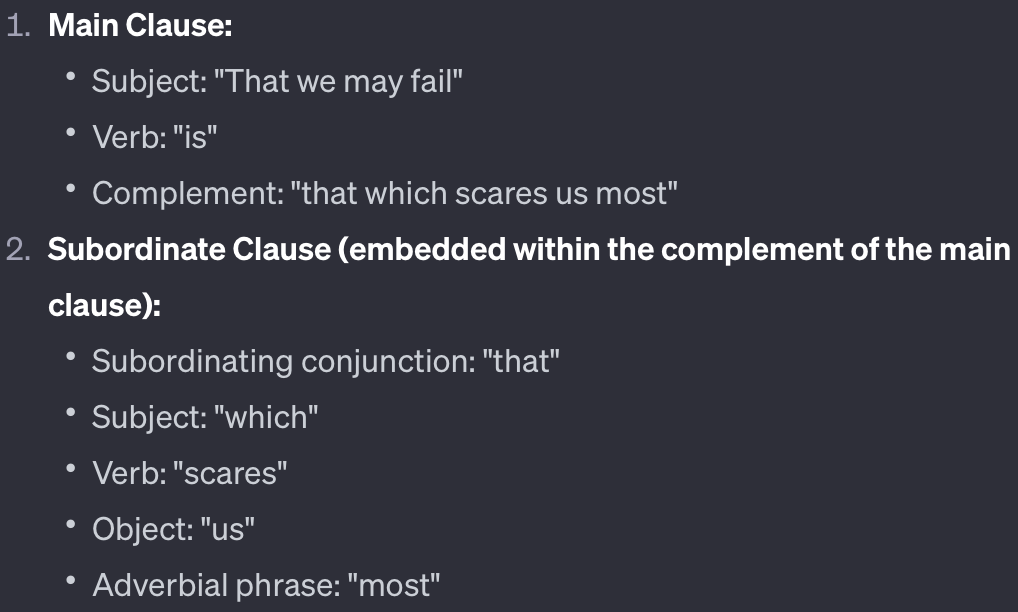
\includegraphics[width=0.7\textwidth]{sen4.png} 
  \caption{sentence 4}
\end{figure}


Sentence 4 was parsed incorrectly. In English, for emphasis, one may begin the utterance with the clausal compliment ('that we may fail') - this does not make it the subject. Interestingly, the same sentence in the other order (sentence 5) is correctly interpreted). 
\\
\subsubsection{}	%sentence 5
Sentence 5: "That which scares us most is that we may fail." \\
\begin{figure}[H]
  \centering
  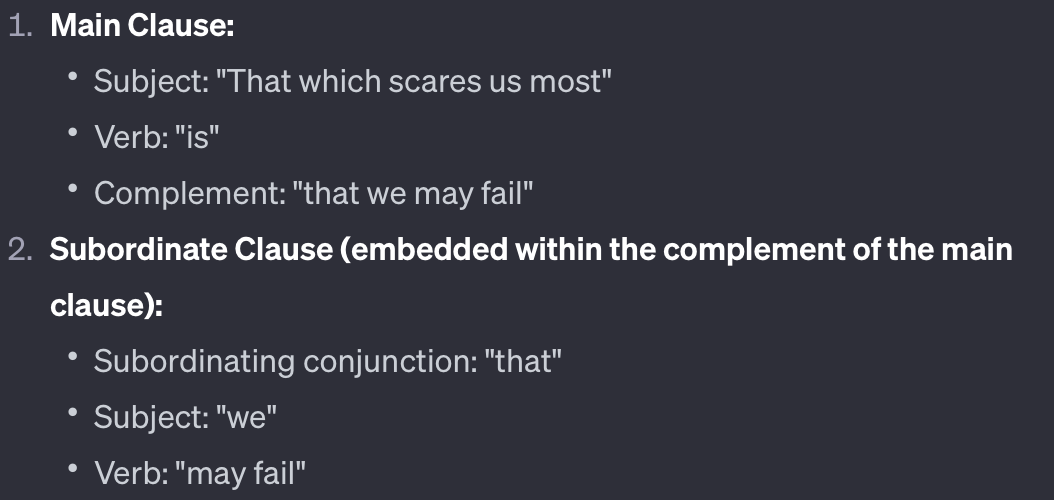
\includegraphics[width=0.7\textwidth]{sen5.png} 
  \caption{sentence 5}
\end{figure}


Perfect. \\
\subsubsection{}	%sentence 6
Sentence 6: "Whether she likes it is what we're worried about." \\
\begin{figure}[H]
  \centering
  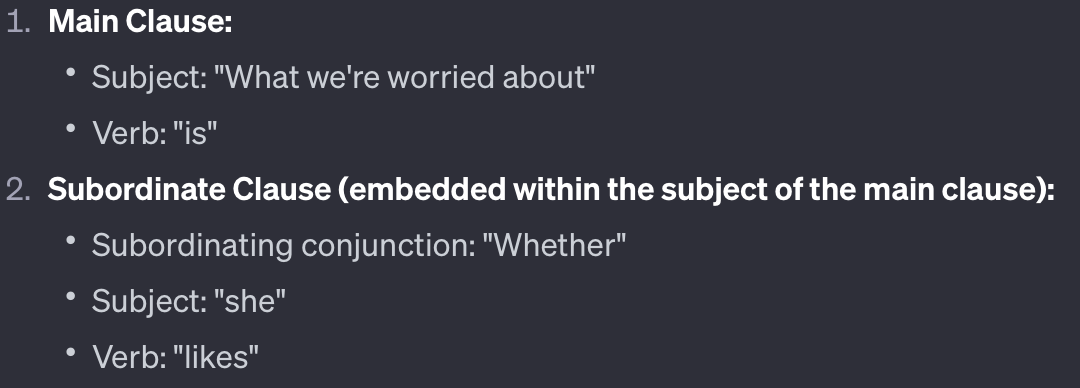
\includegraphics[width=0.7\textwidth]{sen6.png} 
  \caption{sentence 6}
\end{figure}


Incomplete but good job GPT. Interestingly, they weren't thrown off this time with the sentence-initial compliment, probably because 'whether' typically introduces a clausal compliment.  
\\
\subsubsection{}	%sentence 7
Sentence 7: "Thinking I'd already missed the train, I quickly dropped the pace and leisurely meandered along the quaint streets of the old town." \\
\begin{figure}[H]
  \centering

  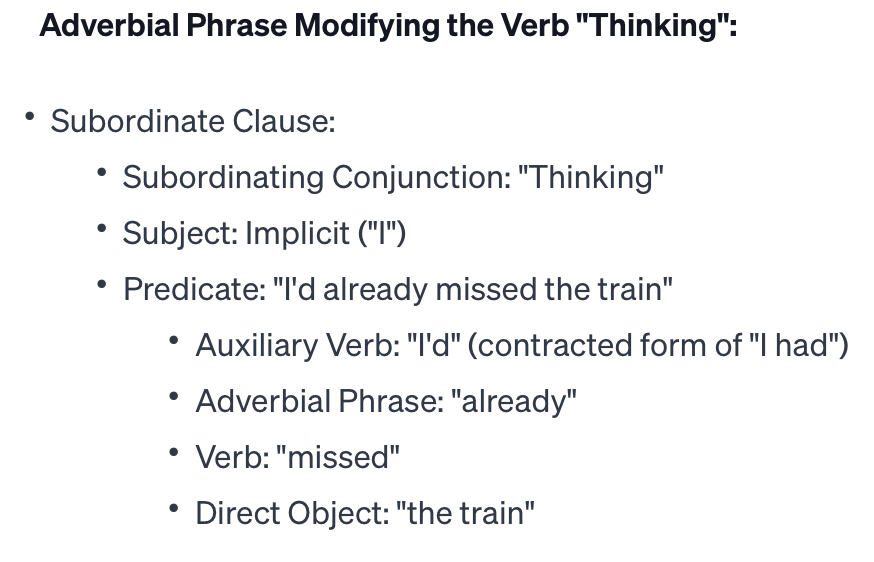
\includegraphics[width=0.45\textwidth]{sen7a.png}

  \vspace{10pt} % Adjust the vertical space between the images

  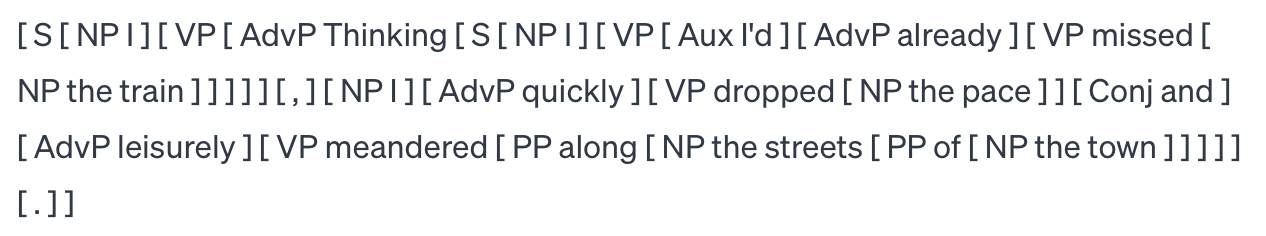
\includegraphics[width=0.8\textwidth]{sen7b.png}

  \caption{sentence 7}
  \label{fig:overall}
\end{figure}


GPT did a good job with this sentence. I added a screenshot of just a part of the detailed description, where it even describes the implicit subject "I" in the adverbial phrase "Thinking..."  \\
I also prompted for a parsing in bracket notation and it seems quite good. \\

\subsubsection{}	%sentence 8
Sentence 8: "She said she thought she knew his intent but she assumed he knew too." \\
\begin{figure}[H]
  \centering
  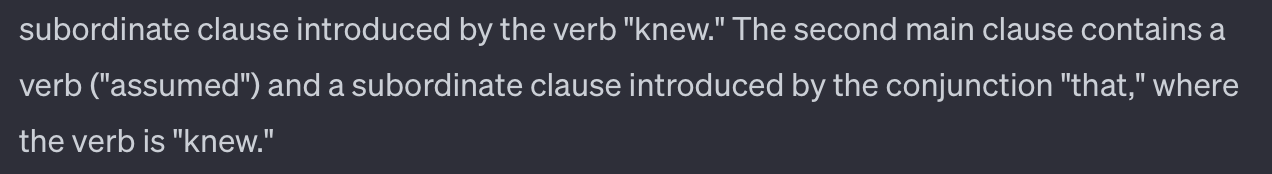
\includegraphics[width=0.7\textwidth]{sen8.png} 
  \caption{sentence 8}
\end{figure}


GPT parsed this sentence perfectly, but then in it's summary it says "subordinate clause introduced by the conjunction 'that'" - but this isn't in the sentence I gave - here we can see that it so expects something it just assumes it's there. 

\subsubsection{}	%sentence 9
Sentence 8: "Wenn hinter Fliegen Fliegen fliegen, fliegen Fliegen Fliegen nach." \\
\begin{figure}[H]
  \centering
  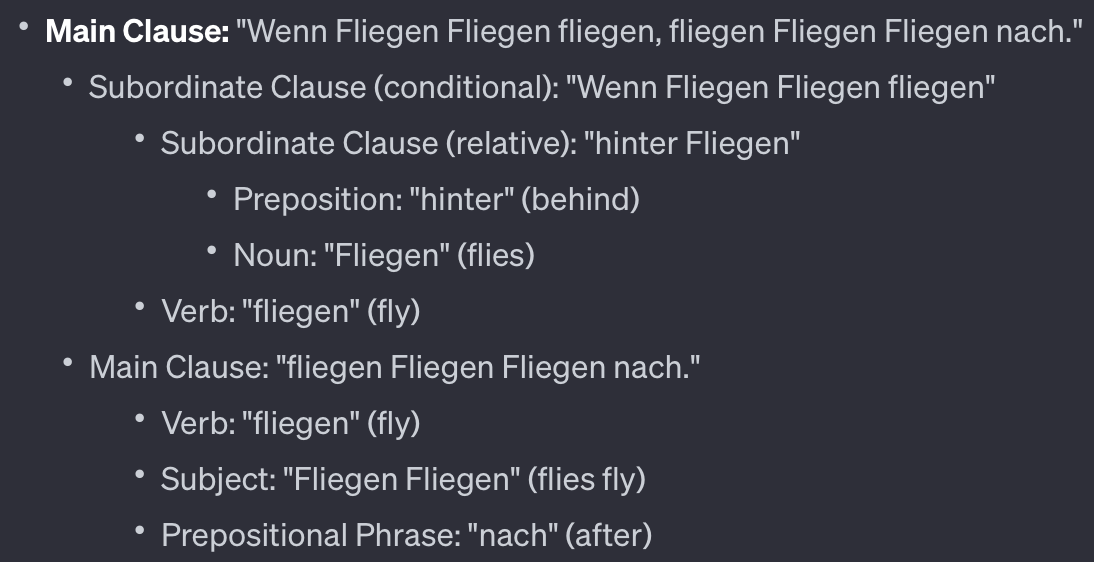
\includegraphics[width=0.7\textwidth]{sen9.png} 
  \caption{sentence 9}
\end{figure}


GPT knows this is a play on words (and must've read about it many times on the internet) and yet fails miserably to identify proper subjects and objects. 
\\ \\
\textbf{4.1 b)} \\ \\
When asked to draw syntactic tree graphs, GPT first draws a simplified graph with some of the constituents missing. When prompted to draw a detailed tree, the provide code that looks like this: 
\begin{figure}[H]
  \centering
  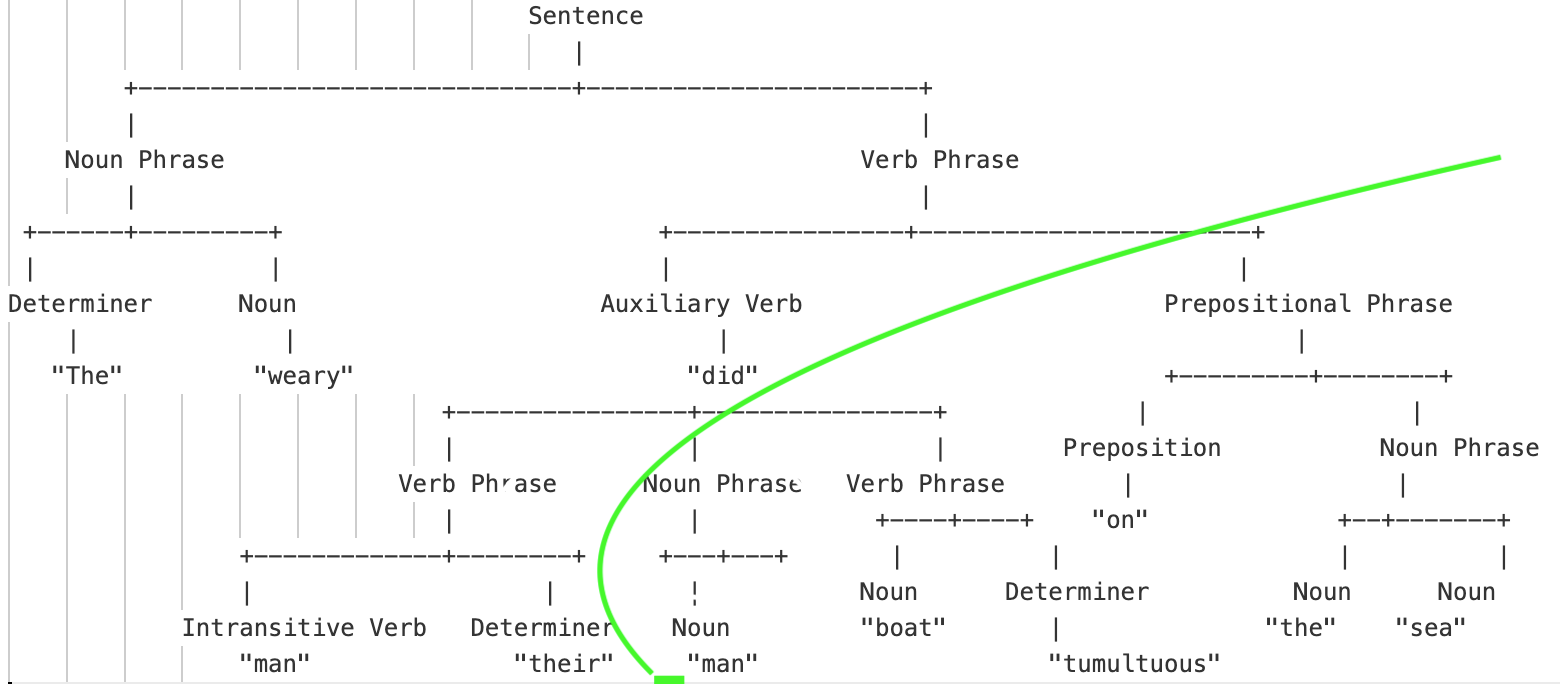
\includegraphics[width=1\textwidth]{b3.png} 
  \caption{GPT tree sentence 3}
\end{figure}
This is interesting because GPT did quite a good job, and then failed miserably (like really random...) Everything is fine except the bottom right corner (marked with green line), where GPT starts making stuff up, like the Verb Phrase consisting of 'boat tumultuous"!

\begin{figure}[H]
  \centering
  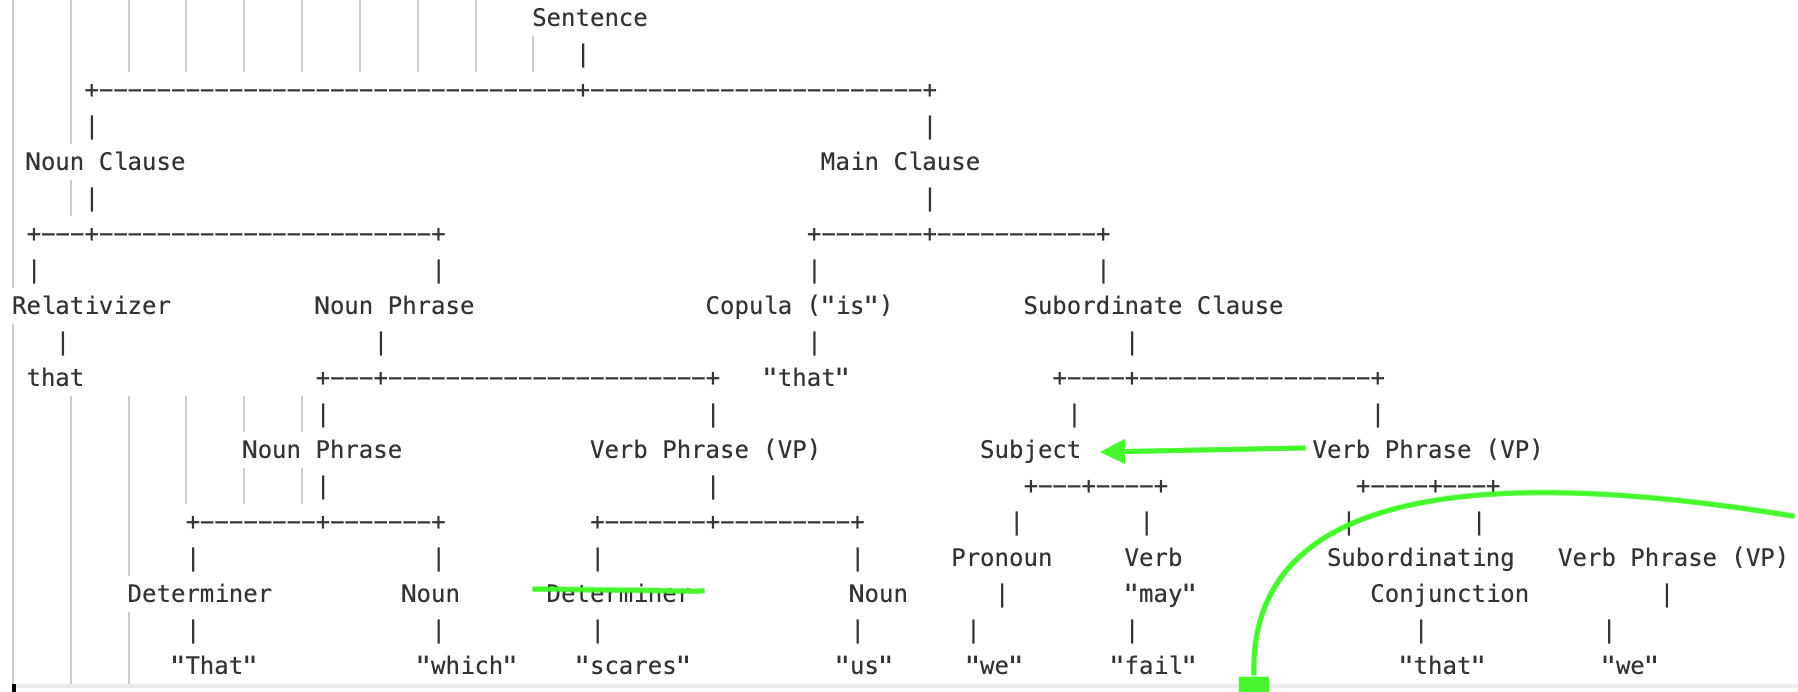
\includegraphics[width=1\textwidth]{b5.png} 
  \caption{GPT tree sentence 5}
\end{figure}
Again GPT does really well except for the bottom right corner (what is it with that, like a grey zone for GPT, it knows something must come there but doesn't know what...) In this case it should've just been left blank, it didn't need another branch there. And the "subject" branch should've read "verb phrase". 

\subsection{}	% 4.2

\subsubsection{}	%sentence 1
Sentence 1: rewrite the following sentence in reported speech. 'I'm now looking to somehow find a somewhat more fitting replacement to tackle the tedious task at hand.' \\
\begin{figure}[H]
  \centering
  
\includegraphics[width=0.7\textwidth]{2sen1.png} 
  \caption{sentence 1}
\end{figure}
GPT correctly wrote the sentence in reported speech, and for some reason chose a masculine third person. They also replaced "fitting" with a synonym, "suitable", without me asking it to do that. 

\subsubsection{}	%sentence 2
Sentence 2: rewrite the following sentence in reported speech. 'I'm now looking to somehow lessen this burden for my family in this country of mine' \\
\begin{figure}[H]
  \centering
  
\includegraphics[width=0.7\textwidth]{2sen2.png} 
  \caption{sentence 2}
\end{figure}
Again a grammatically correct sentence, this time both genders are given as options. I like that it correctly changed the deictic expressions (this to that) for reported speech. 

\subsubsection{}	%sentence 3
Sentence 3: now rewrite this sentence in direct speech: "She said they were only coming tomorrow." \\
\begin{figure}[H]
  \centering
  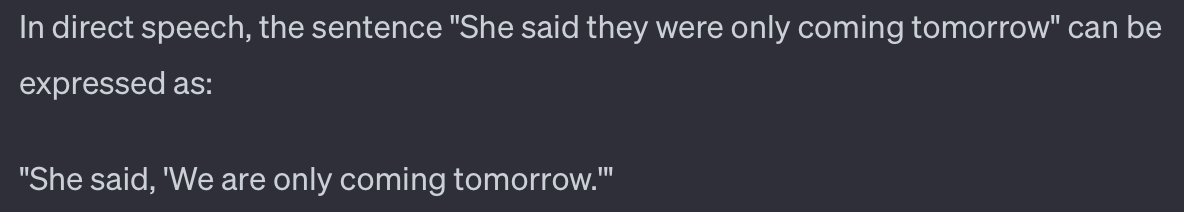
\includegraphics[width=0.7\textwidth]{2sen3.png} 
  \caption{sentence 3}
\end{figure}
Great job, GPT! They even got the tense change right from "she said they were" to "we are".

\subsubsection{}	%sentence 4
\begin{figure}[H]
  \centering
  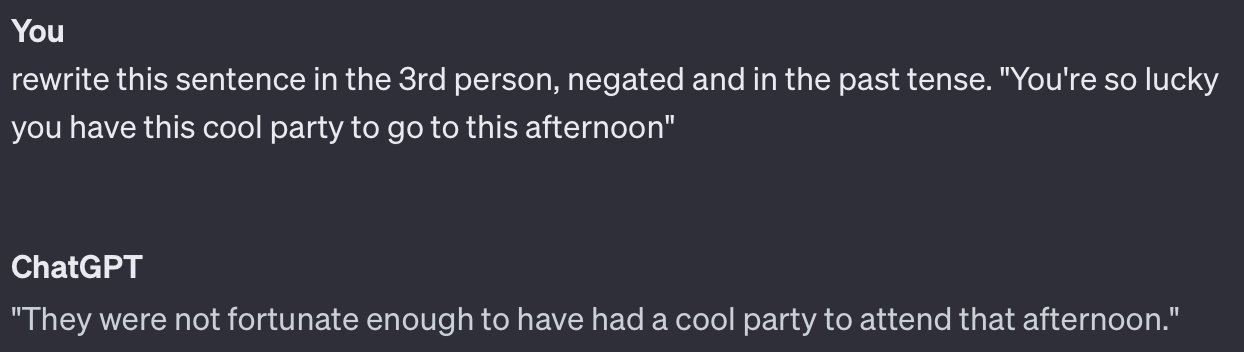
\includegraphics[width=0.7\textwidth]{2sen4.png} 
  \caption{sentence 4}
\end{figure}
Not bad! I was expecting 'he' or 'she' but 'they' is perfectly fine even for singular 3rd person in English. 

\subsubsection{}	%sentence 5
\begin{figure}[H]
  \centering
  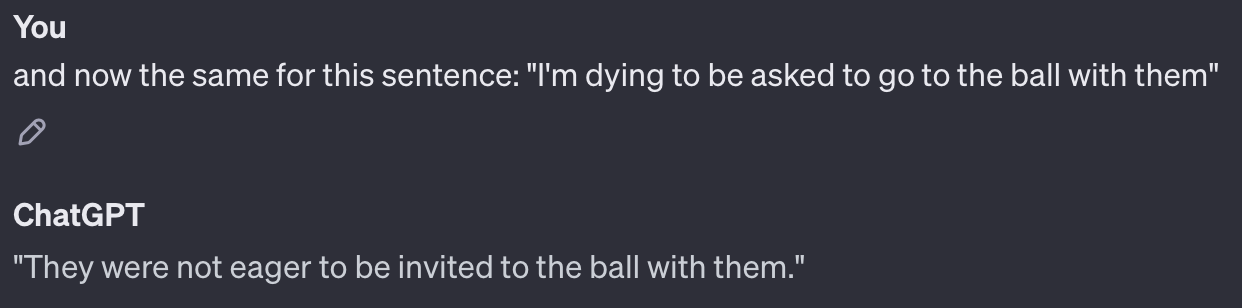
\includegraphics[width=0.7\textwidth]{2sen5.png} 
  \caption{sentence 5}
\end{figure}
Perfect. I like how "i'm dying to" was changed to "they were not eager to", as negating "dying to" would sound odd!

\subsubsection{}	%sentence 6
\begin{figure}[H]
  \centering
  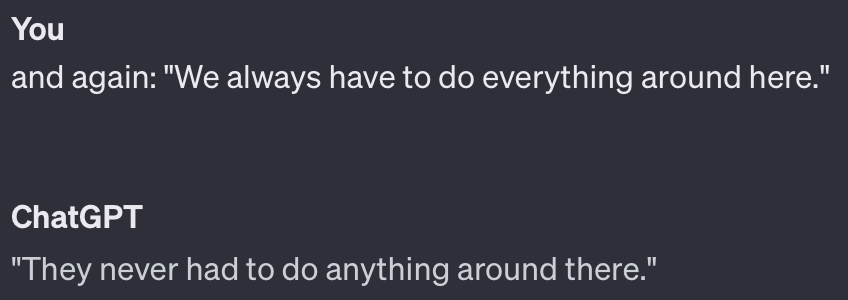
\includegraphics[width=0.5\textwidth]{2sen6.png} 
  \caption{sentence 6}
\end{figure}
This one takes the cake! The deixis and the indefinite pronouns were correctly converted. 

\subsubsection{}	%sentence 7
\begin{figure}[H]
  \centering
  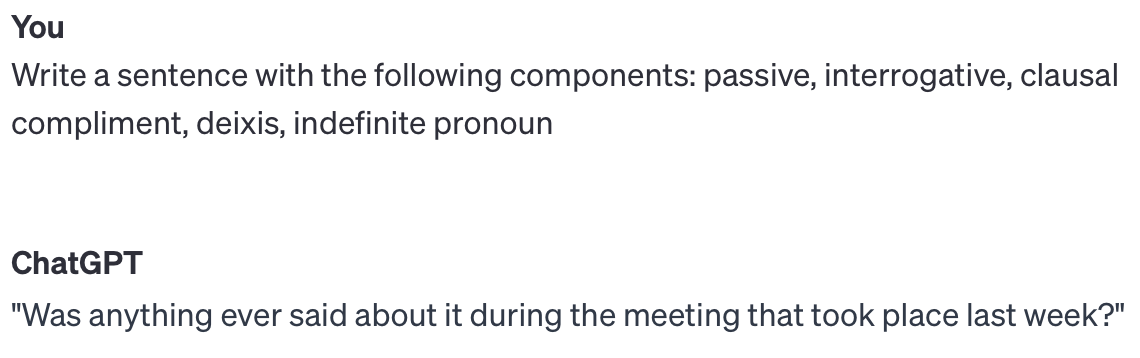
\includegraphics[width=0.7\textwidth]{2sen7.png} 
  \caption{sentence 7}
\end{figure}
Impressive. 

\subsubsection{}	%sentence 8
\begin{figure}[H]
  \centering
  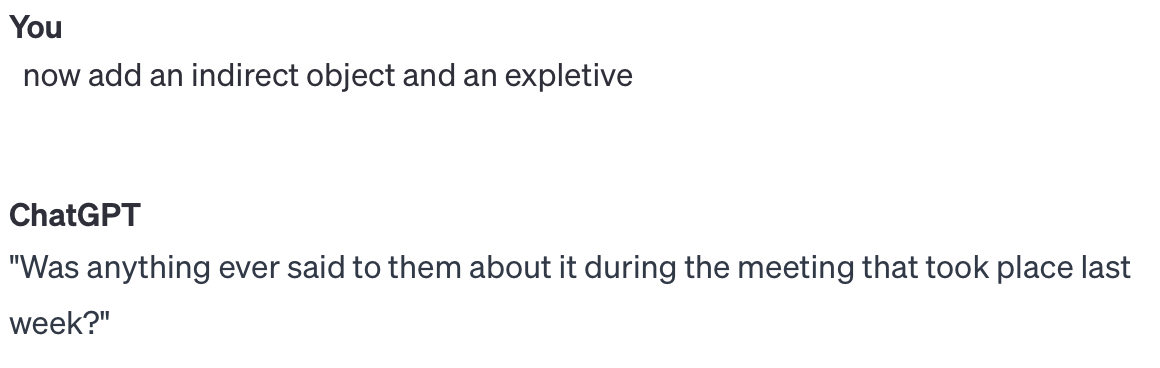
\includegraphics[width=0.7\textwidth]{2sen8.png} 
  \caption{sentence 8}
\end{figure}
Nice addition of indirect object - the expletive is missing though. 

\subsubsection{}	%sentence 9
\begin{figure}[H]
  \centering
  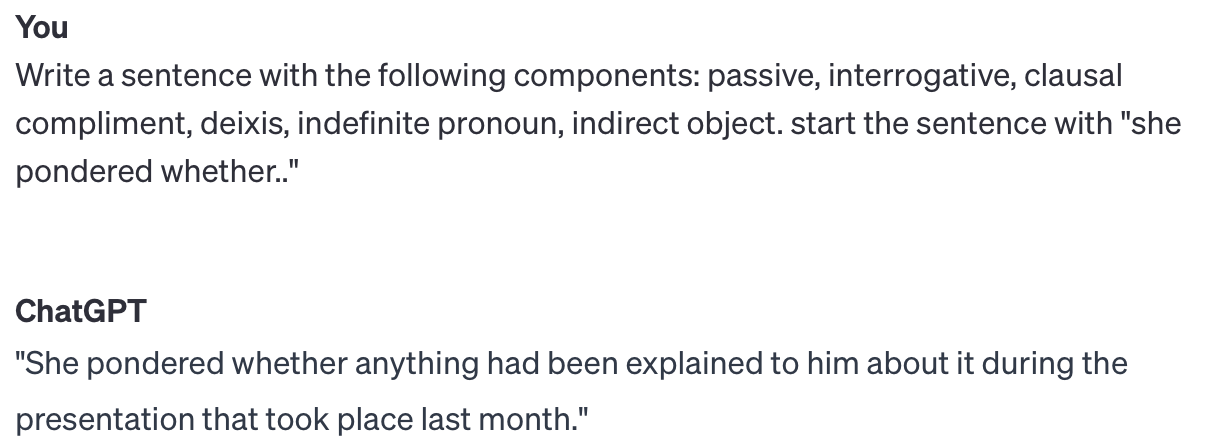
\includegraphics[width=0.7\textwidth]{2sen9.png} 
  \caption{sentence 9}
\end{figure}
Couldn't have done it better :)

\subsection{}		%4.3
\subsubsection{}	%sentence 1
\begin{figure}[H]
  \centering
  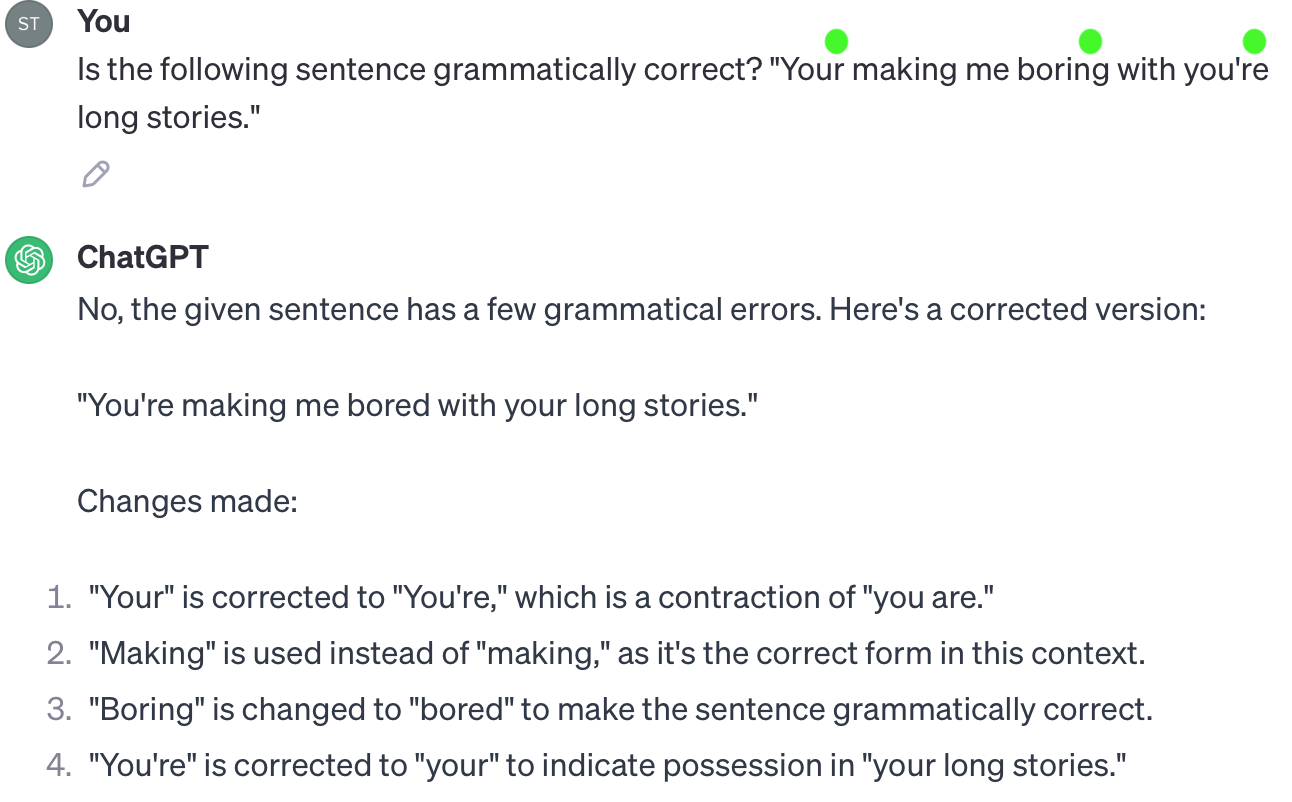
\includegraphics[width=0.7\textwidth]{3sen1.png} 
  \caption{sentence 1}
\end{figure}
Perfect. It picked up all 3 errors. It somehow added a superfluous point (making instead of making) in it's summary. 

\subsubsection{}	%sentence 2
\begin{figure}[H]
  \centering
  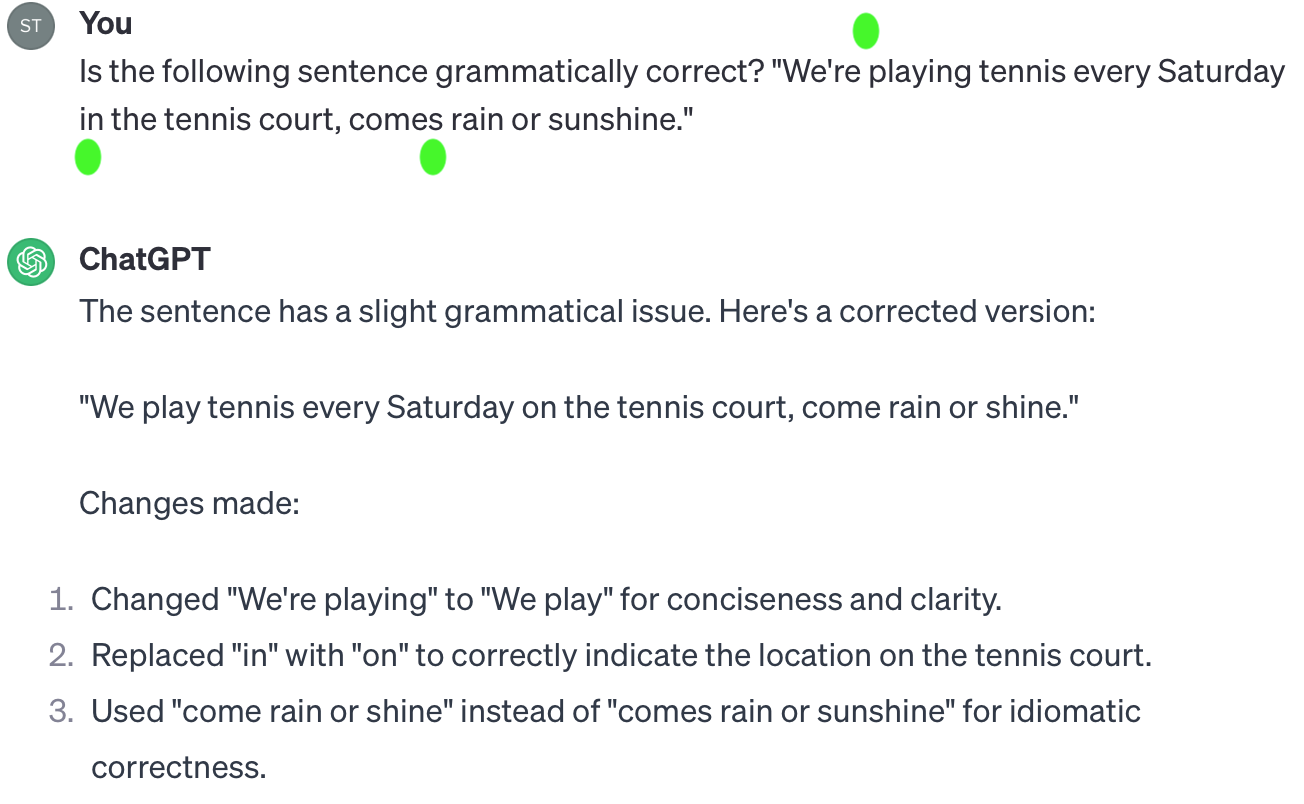
\includegraphics[width=0.7\textwidth]{3sen2.png} 
  \caption{sentence 2}
\end{figure}
Great. I like that it corrected the tense due to the repetitiveness of the action (every Saturday). It also picked up on the wrong preposition used with a tennis court and most interestingly, the subjunctive 'come' instead of 'comes', as this is a set expression in English. 

\subsubsection{}	%sentence 3
\begin{figure}[H]
  \centering
  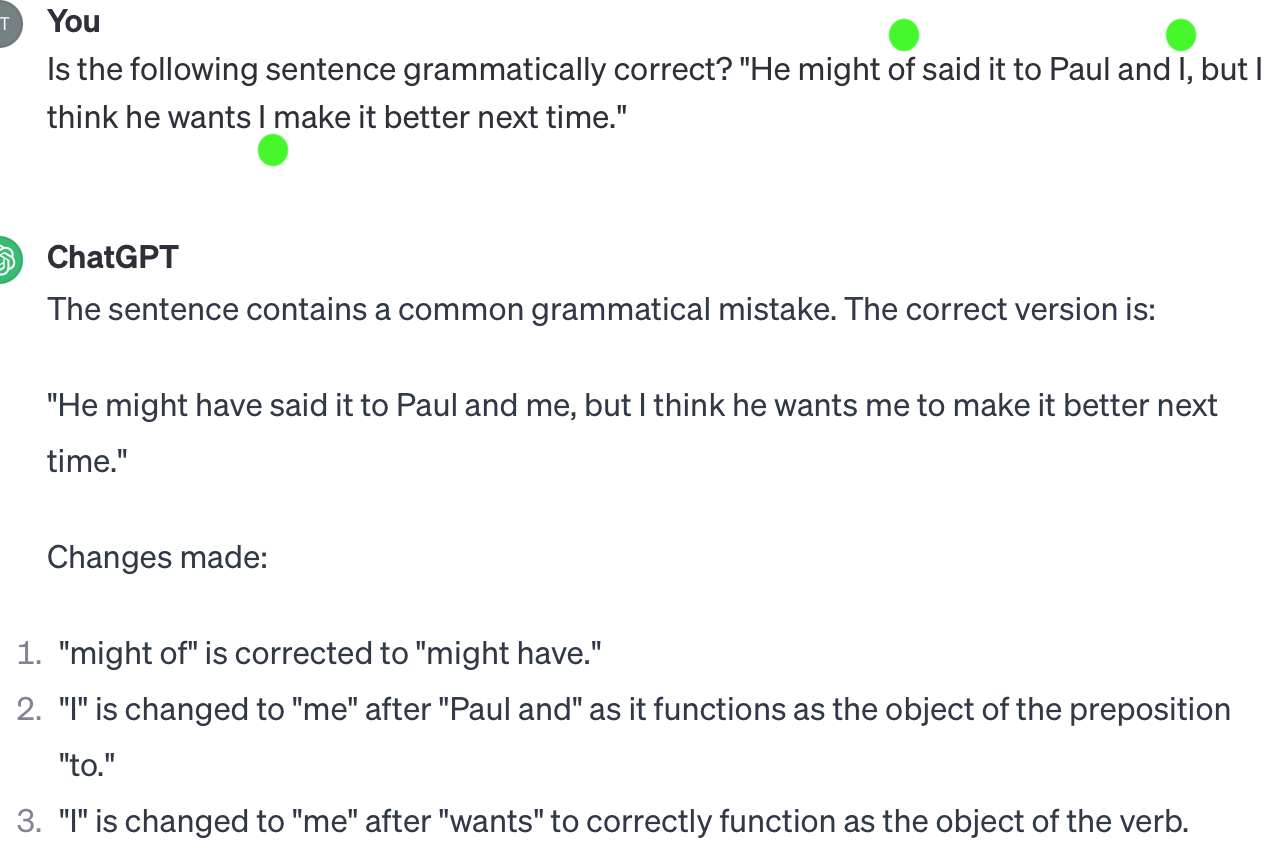
\includegraphics[width=0.7\textwidth]{3sen3.png} 
  \caption{sentence 3}
\end{figure}
Quite impressive, perfectly done again. 


\subsection{}




\end{document}